\documentclass[tikz,border=10pt]{standalone}
\usepackage{amsmath,amssymb}
\usetikzlibrary{arrows.meta,positioning,calc,decorations.pathmorphing}

\newcommand{\ord}{\operatorname{ord}}

\begin{document}
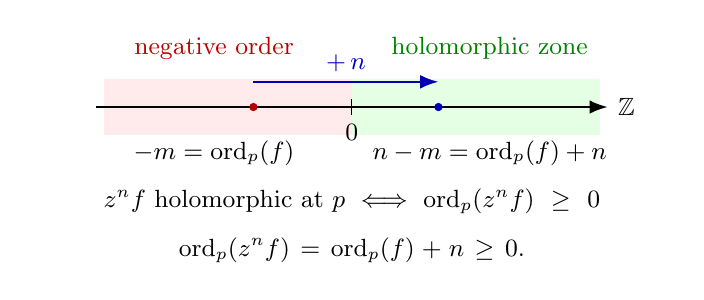
\begin{tikzpicture}[
		>=Latex,
		font=\small,
		panel/.style={
			rounded corners=5pt, thick},
		title/.style={font=\large\bfseries},
		point/.style={circle, fill=black, inner sep=1.4pt},
		good/.style={green!50!black, thick},
		bad/.style={red!70!black, thick},
		flow/.style={->, thick, black},
		every node/.style={align=center}
		]
		
		% shaded regions
		\fill[red!8] (-3.15,-0.15) rectangle (0,0.55);
		\fill[green!10] (0,-0.15) rectangle (3.15,0.55);
		
		% axis
		\draw[thick,->] (-3.25,0.2) -- (3.25,0.2) node[right] {$\mathbb{Z}$};
		\draw (0,0.1) -- (0,0.3);
		\node[below] at (0,0.1) {$0$};
		\node[below] at (-1.75,-0.1) {$-m=\ord_p(f)$};
		\node[below] at (1.75,-0.1) {$n-m=\ord_p(f)+n$};
		
		% points and arrow
		\fill[red!70!black] (-1.25,0.2) circle (1.5pt);
		\fill[blue!70!black] (1.1,0.2) circle (1.5pt);
		\draw[flow,blue!70!black] (-1.25,0.52) -- node[above] {$+\,n$} (1.1,0.52);
		
		\node[red!75!black] at (-1.75,0.95) {negative order};
		\node[green!50!black] at (1.75,0.95) {holomorphic zone};
		
		\node[text width=8.0cm] at (0,-1)
		{$z^n f$ holomorphic at $p$
			\;$\Longleftrightarrow$\;
			$\ord_p(z^n f)\ge 0$};
		
		\node[text width=5.0cm] at (0,-1.62)
		{$\ord_p(z^n f)=\ord_p(f)+n\ge 0$.};
\end{tikzpicture}
\end{document}